\documentclass{article}
\usepackage{graphicx} 

\setlength{\parindent}{15pt}
\setlength{\parskip}{5pt}

\usepackage[margin=1.5in]{geometry}
\usepackage{amssymb}
\usepackage{amsmath}
\usepackage{mathtools}
\usepackage{xcolor}
\usepackage{cancel}
\usepackage{centernot}
\usepackage{nicefrac}
\usepackage{bm}
\usepackage{indentfirst}
\usepackage{float}
\usepackage[round]{natbib} 
\usepackage[hidelinks]{hyperref}
\usepackage{enumerate}
\usepackage{titling}
\usepackage{enumitem}
\usepackage{parskip}
\usepackage{subcaption}

\setlist[itemize]{label=\textendash}

\newenvironment{answer}{\par\vspace{0.8em}\textbf{A:}}{\par}
\newcommand{\red}[1]{\textcolor{red}{#1}}
\newcommand{\blue}[1]{\textcolor{blue}{#1}}
\newcommand{\fa}{\text{ for all }} 
\newcommand{\ex}{\text{ there exists }}
\newcommand{\st}{\text{ such that }}
\newcommand{\for}{\text{ for }}
\newcommand{\andt}{\text{ and }}
\newcommand{\ort}{\text{ or }}
\newcommand{\ift}{\text{ if }}
\newcommand{\where}{\text{ where }}
\newcommand{\but}{\text{ but }}
\newcommand{\nat}{\mathbb{N}}
\newcommand{\rat}{\mathbb{Q}}
\newcommand{\com}{\mathbb{C}}
\newcommand{\real}{\mathbb{R}}
\newcommand{\norm}[1]{\lVert#1\rVert}
\newcommand{\abs}[1]{\lvert#1\rvert}
\newcommand{\corr}{\rightrightarrows}
\newcommand{\ul}{\underline}
\newcommand{\bft}{\textbf}
\newcommand{\itt}{\textit}
\newcommand{\E}{\mathbb{E}}
\newcommand{\Prob}{\operatorname{P}}
\newcommand{\Var}{\operatorname{Var}}
\newcommand{\Cov}{\operatorname{Cov}}
\newcommand{\Unif}{\operatorname{Unif}}
\newcommand{\Bias}{\operatorname{Bias}}
\newcommand{\N}{\operatorname{N}}
\newcommand{\MSE}{\operatorname{MSE}}
\newcommand{\iffs}{\Leftrightarrow}
\newcommand{\prefeq}{\trianglerighteq}
\newcommand{\pref}{\triangleright}
\newcommand{\indiff}{\mathrel{\triangleright\triangleleft}}

\title{Current analysis}
\date{\today}

\begin{document}

\maketitle

\section*{Original hypotheses}

Some original hypotheses from drafting the Prolific survey, for why redistributive preferences might change as one ages:
\begin{enumerate}
    \item Income insurance
    \begin{enumerate}
        \item Present financial/employment insecurity
        \item Longer-term income/career uncertainty
        \item Uncertainty about the future state of the world (housing, climate, AI)
    \end{enumerate}
    \item Consumption smoothing
    \item Myopia or time-discounting
    \item Lived experience
    \begin{enumerate}
        \item Misperceived future income needs
        \item Moving up/down the income ladder
        \item Observing others' paths
        \item Experiencing taxation first-hand
    \end{enumerate}
    \item Disagreement about incentive effects
    \item Different preferences for consumption/leisure
    \item Differences in individualism/universalism
\end{enumerate}

\paragraph{Suggestive results:} Combining age gradients in beliefs/circumstances with correlations between beliefs/circumstances and redistributive preferences gives us suggestive evidence. For example, we know from the regressions in figure \ref{fig:baseline-ologit} that belief that the economic game is zero-sum correlates with support redistribution, and from our cohort analysis (age gradient tex file), young people tend to have more zero-sum beliefs. Similarly, belief that DEI initiatives are positive-sum, pessimism about mobility, non-materialism (satisfied with basics, salary not important), myopia (taking less money now over more money later, current desires over future needs, see fig \ref{fig:progressivity-myopia}), financial worries, and worries about climate are all correlated with both youth and desired tax progressivity. We also find that experiencing mobility (income now greater than income growing up) decreases demand for redistribution and correlates positively with age, but that this variable is insignificant in regressions with the other covariates. Although beliefs about incentive effects of taxation strongly predict redistributive preferences, these beliefs tend not to be strongly correlated with age in our survey.

We also find that young people may actually overestimate their future income needs (fig \ref{fig:needs}), and that expected income growth may reduce demand for redistribution (fig \ref{fig:shouldconcern-hhincgrowth40s}), pushing against the consumption smoothing hypothesis. Speaking to the final hypotheses, a proxy for materialism (ranksalary + satisfiedbasics) and proxies for universalism/generosity (stranger100, friend100) tend not to be significant in larger regressions.
\blue{Combined, these findings tell us something about hypotheses 1a, 1c, 2, 3, 4a, 4b, 5, 6, and 7. 1b is explored in the next section. Lived experiences such as 4c-4d are less-analyzed.}

% \subsection*{Evidence}

% \begin{enumerate}
%     \item 
%     \begin{enumerate}
%         \item 
%         \item 
%         \item 
%     \end{enumerate}
%     \item 
%     \item 
%     \item Young people may actually overestimate their future income needs 
% \begin{figure}[H]
%     \centering
%     \begin{subfigure}{.45\textwidth}
%         \centering
%         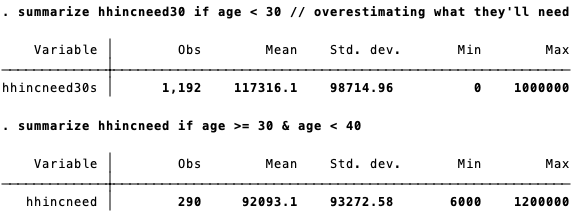
\includegraphics[width=\linewidth]{images/needs30s.png}
%     \end{subfigure}
%     \begin{subfigure}{.45\textwidth}
%         \centering
%         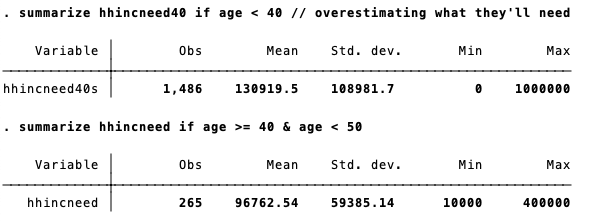
\includegraphics[width=\linewidth]{images/needs40s.png}
%     \end{subfigure}
% \end{figure}
%     \item 
%     \item 
%     \item 
% \end{enumerate}

\section*{Insurance hypothesis}

One core hypothesis is the insurance motive. It seems that, especially for young people, downside income risk is associated with demand for redistribution (fig \ref{fig:progressivity-pinc10low}). 

\paragraph{Moderating beliefs:} Further, a lack of belief in mobility amplifies this correlation (figs \ref{fig:progressivity-yesharder} and \ref{fig:progressivity-notpaid}); if one cannot work hard to guarantee themselves a career/income path, demand for redistribution is more sensitive to risk. Among the young with high income risk and low beliefs in mobility, support for the proposal helping the poor is high and significant (fig \ref{fig:poor-notpaid}), even though the sample size is low.

\paragraph{Suppport by young vs. old for alternative policies:} It seems that older Americans exposed to downside risk favor policies other than redistribution. The young exposed to tail income risk support wealth taxes (fig \ref{fig:young-old-wealthtax-notpaid}) and universal healthcare (fig \ref{fig:young-old-univhealth-notpaid}), but with lower significance than income redistribution. The old exposed to tail income risk instead support lower education expenditures (fig \ref{fig:young-old-fundedu-notpaid}) and \textit{less} trade protectionism (fig \ref{fig:young-old-protecttrade-notpaid}), with decent significance. This could be because education expenditures erode older Americans' wealth/income without much benefit to them, while trade protections are heavily associated with high prices. Further, grouping by mobility beliefs affects the coefficient on income risk for the young and wealth/healthcare, but not for the old and education/trade. This supports the idea that the old care more about preserving their spending power than insuring against uncertain income paths.

\section*{Regression output}

\begin{figure}[H]
    \centering
    \caption{Ologit baselines}
    \begin{subfigure}{.45\textwidth}
        \centering
        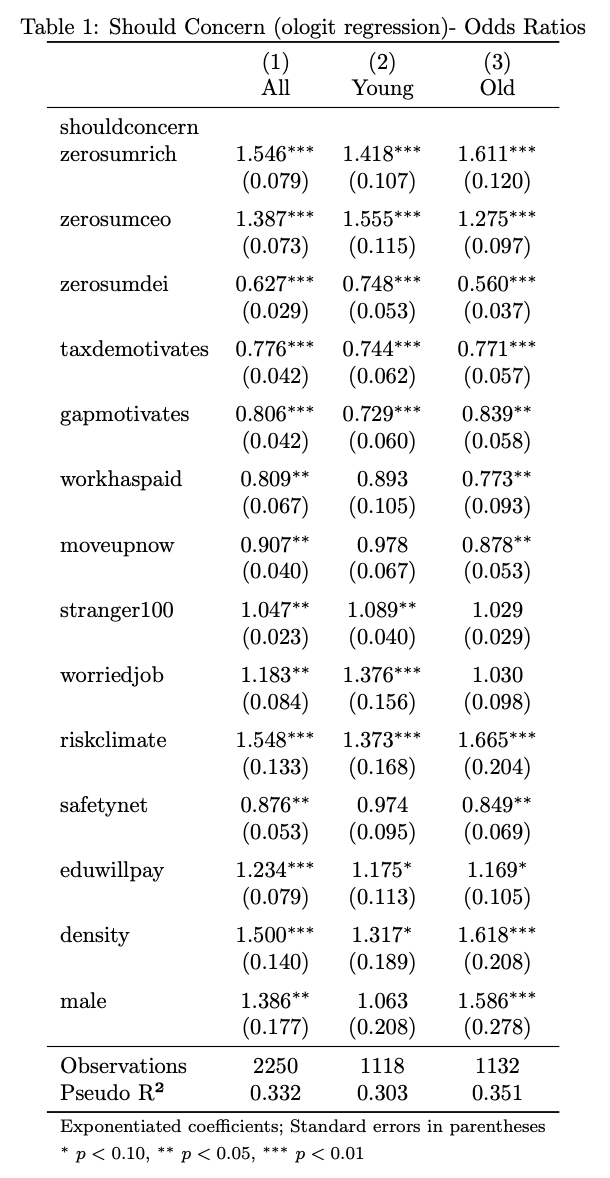
\includegraphics[width=\linewidth]{images/shouldconcern.png}
    \end{subfigure}
    \begin{subfigure}{.45\textwidth}
        \centering
        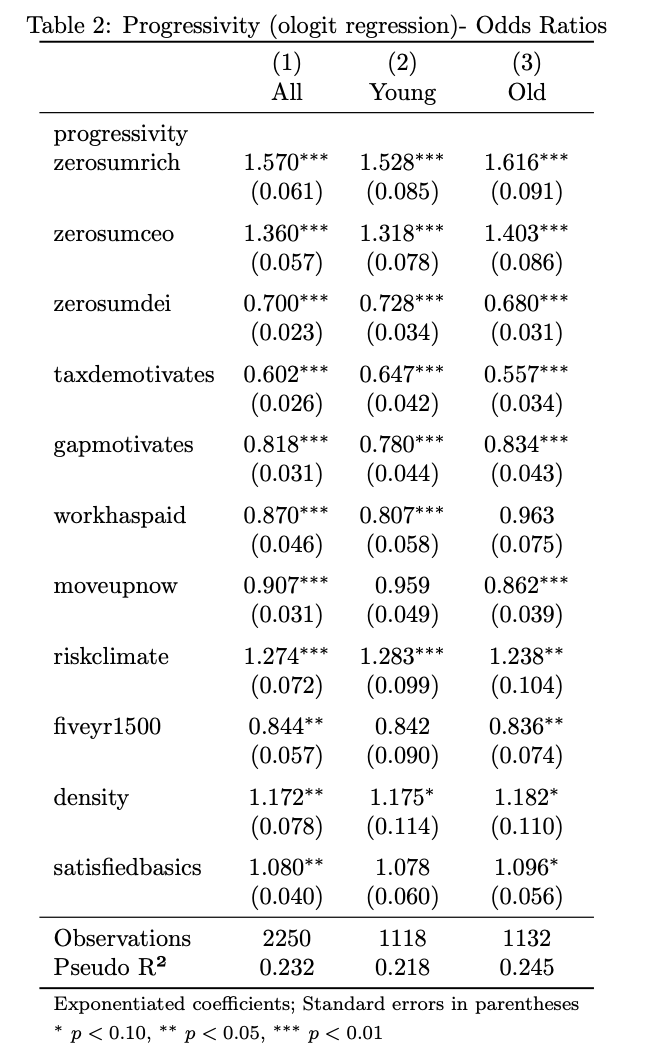
\includegraphics[width=\linewidth]{images/progressivity.png}
    \end{subfigure}
    \label{fig:baseline-ologit}
\end{figure}

\begin{figure}[H]
    \centering
    \caption{Ologit baseline with myopia principal component variable}
    \begin{subfigure}{.65\textwidth}
        \centering
        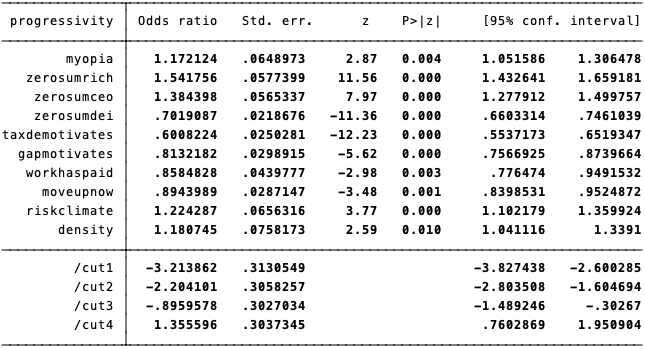
\includegraphics[width=\linewidth]{images/progressivity myopia.png}
    \end{subfigure}
    \label{fig:progressivity-myopia}
\end{figure}

\begin{figure}[H]
    \centering
    \caption{Ologit baseline with variable for expected growth in income needs (needs in 40s divided by current needs)}
    \begin{subfigure}{.65\textwidth}
        \centering
        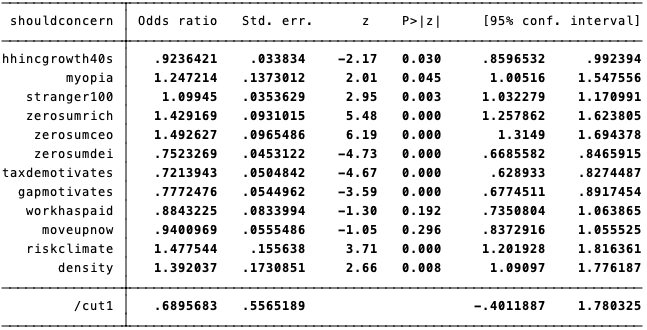
\includegraphics[width=\linewidth]{images/shouldconcern hhincgrowth40s.png}
    \end{subfigure}
    \label{fig:shouldconcern-hhincgrowth40s}
\end{figure}

\begin{figure}[H]
    \centering
    \caption{Progressivity and downside income risk correlation}
    \begin{subfigure}{.45\textwidth}
        \centering
        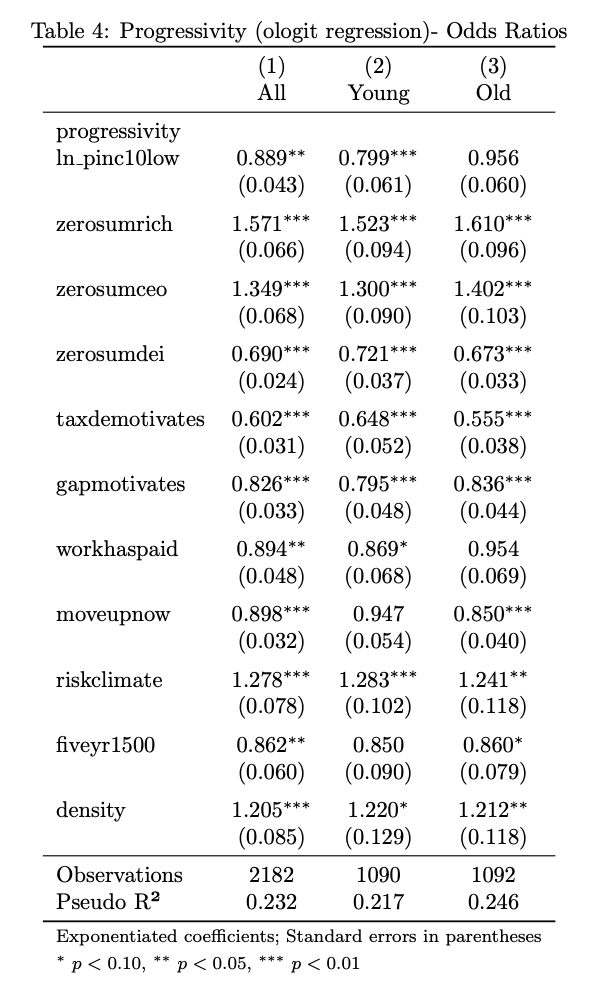
\includegraphics[width=\linewidth]{images/progressivity_pinc10low.png}
    \end{subfigure}
    \label{fig:progressivity-pinc10low}
\end{figure}

\begin{figure}[H]
    \centering
    \caption{Expected vs. realized income needs}
    \begin{subfigure}{.45\textwidth}
        \centering
        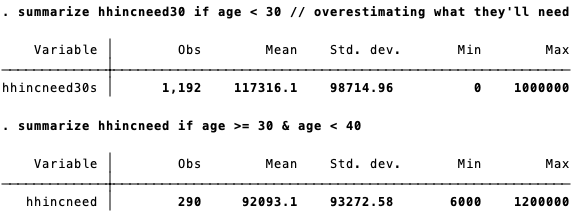
\includegraphics[width=\linewidth]{images/needs30s.png}
    \end{subfigure}
    \begin{subfigure}{.45\textwidth}
        \centering
        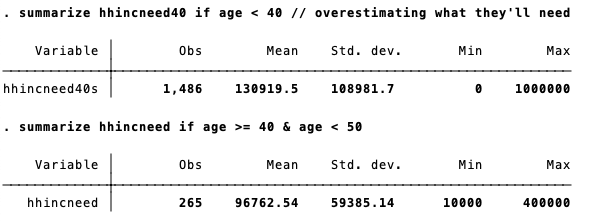
\includegraphics[width=\linewidth]{images/needs40s.png}
    \end{subfigure}
    \label{fig:needs}
\end{figure}

\begin{figure}[H]
    \centering
    \caption{Progressivity and downside risk for two groups: not harder to move up now (LHS) vs. yes harder to move up now (RHS)}
    \begin{subfigure}{.45\textwidth}
        \centering
        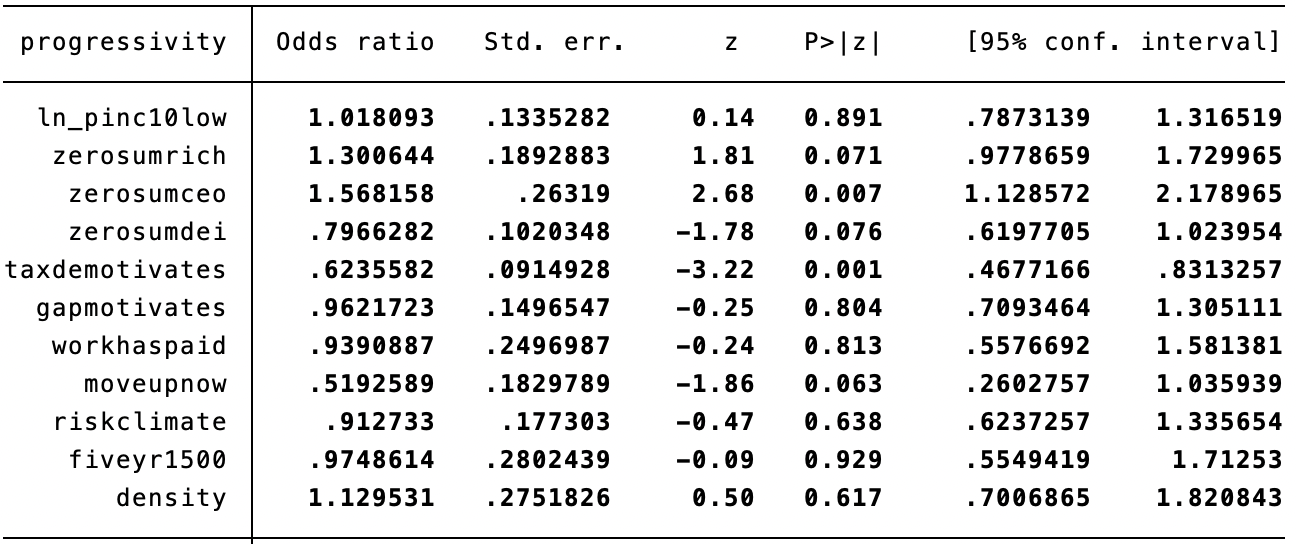
\includegraphics[width=\linewidth]{images/progressivity notharder.png}
    \end{subfigure}
    \begin{subfigure}{.45\textwidth}
        \centering
        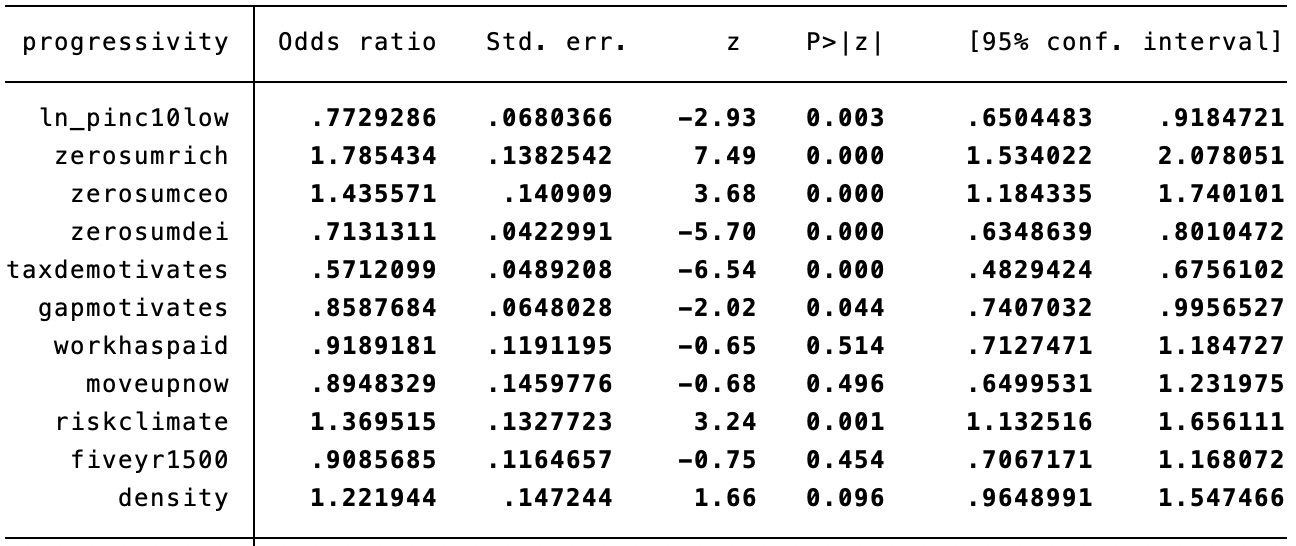
\includegraphics[width=\linewidth]{images/progressivity yesharder.png}
    \end{subfigure}
    \label{fig:progressivity-yesharder}
\end{figure}

\begin{figure}[H]
    \centering
    \caption{Progressivity and downside risk for two groups: hard work has paid off (LHS) vs. hard work has not paid off (RHS)}
    \begin{subfigure}{.45\textwidth}
        \centering
        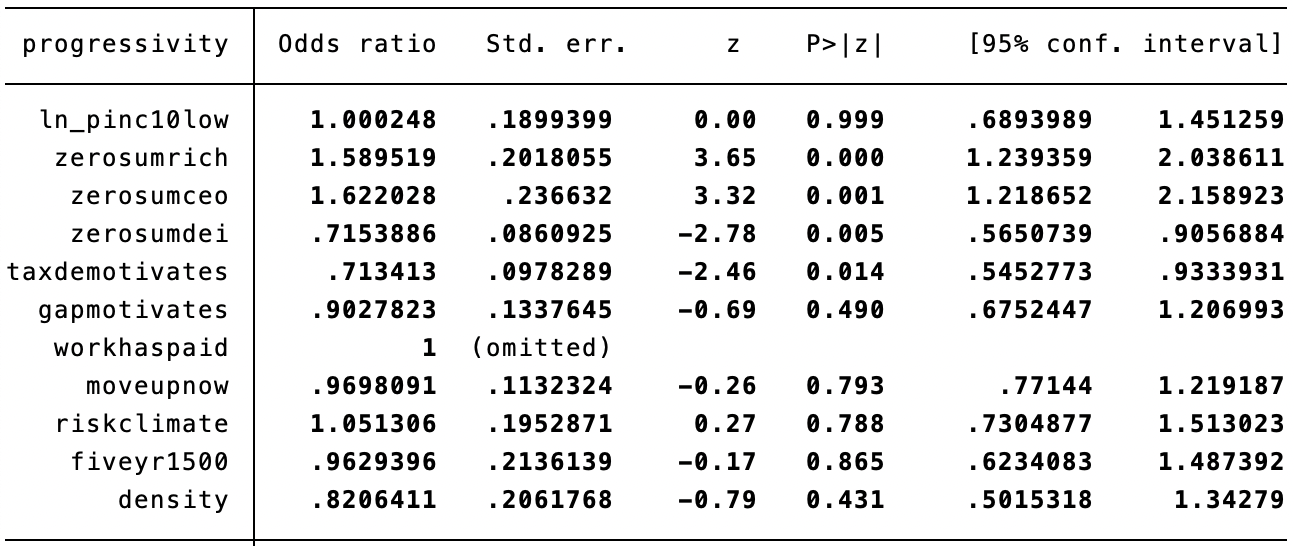
\includegraphics[width=\linewidth]{images/progressivity yespaid.png}
    \end{subfigure}
    \begin{subfigure}{.45\textwidth}
        \centering
        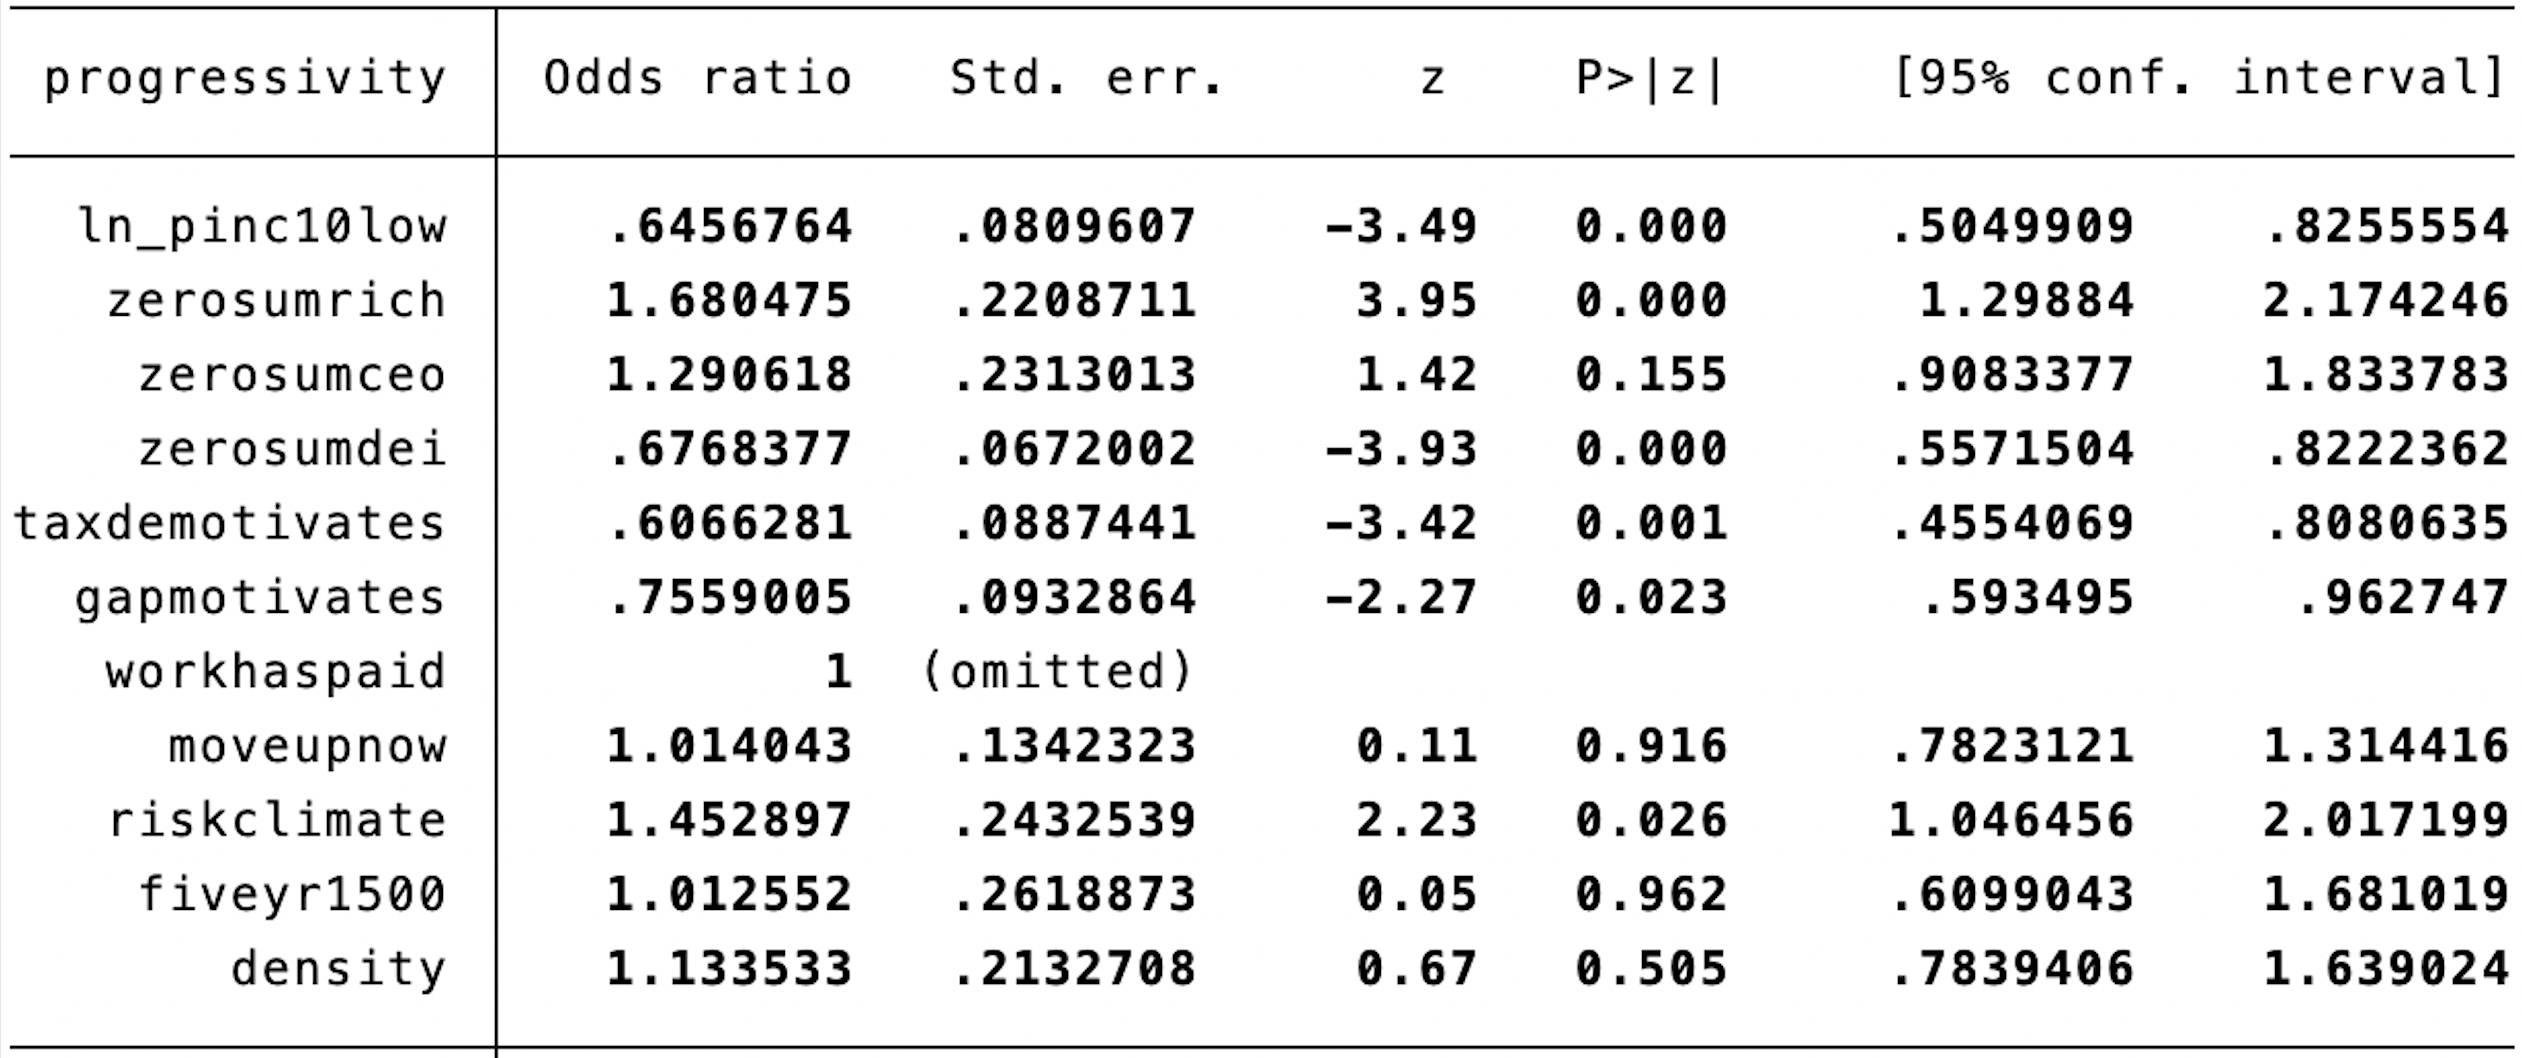
\includegraphics[width=\linewidth]{images/progressivity notpaid.png}
    \end{subfigure}
    \label{fig:progressivity-notpaid}
\end{figure}

\begin{figure}[H]
    \centering
    \caption{Policy supporting poor and downside risk for two groups: all participants (LHS) vs. work has not paid off (RHS)}
    \begin{subfigure}{.45\textwidth}
        \centering
        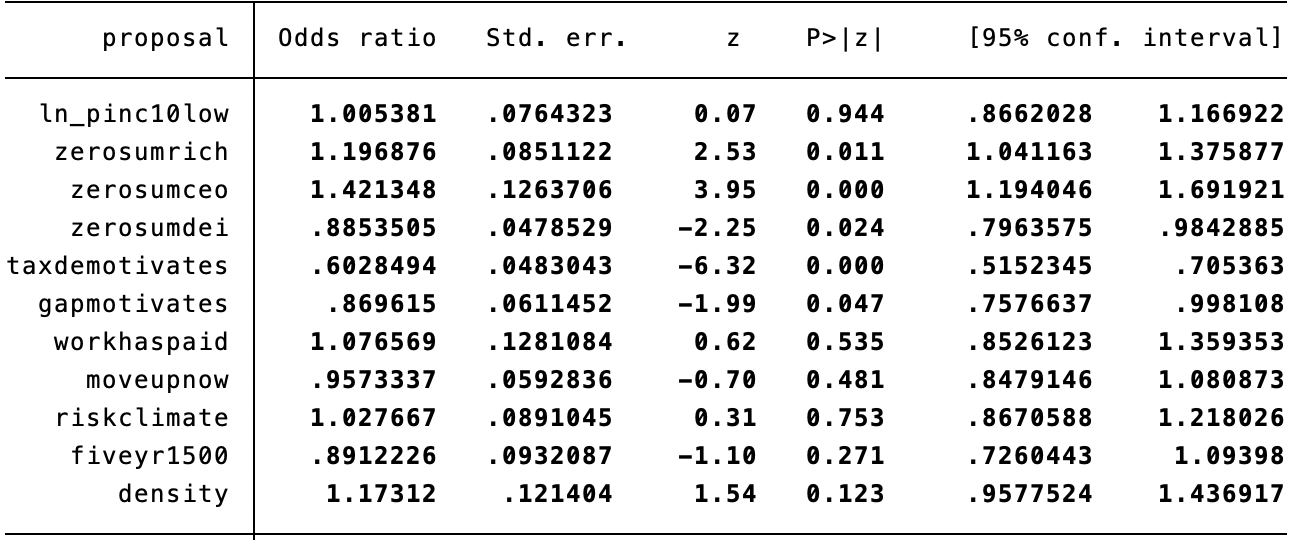
\includegraphics[width=\linewidth]{images/poor baseline.png}
    \end{subfigure}
    \begin{subfigure}{.45\textwidth}
        \centering
        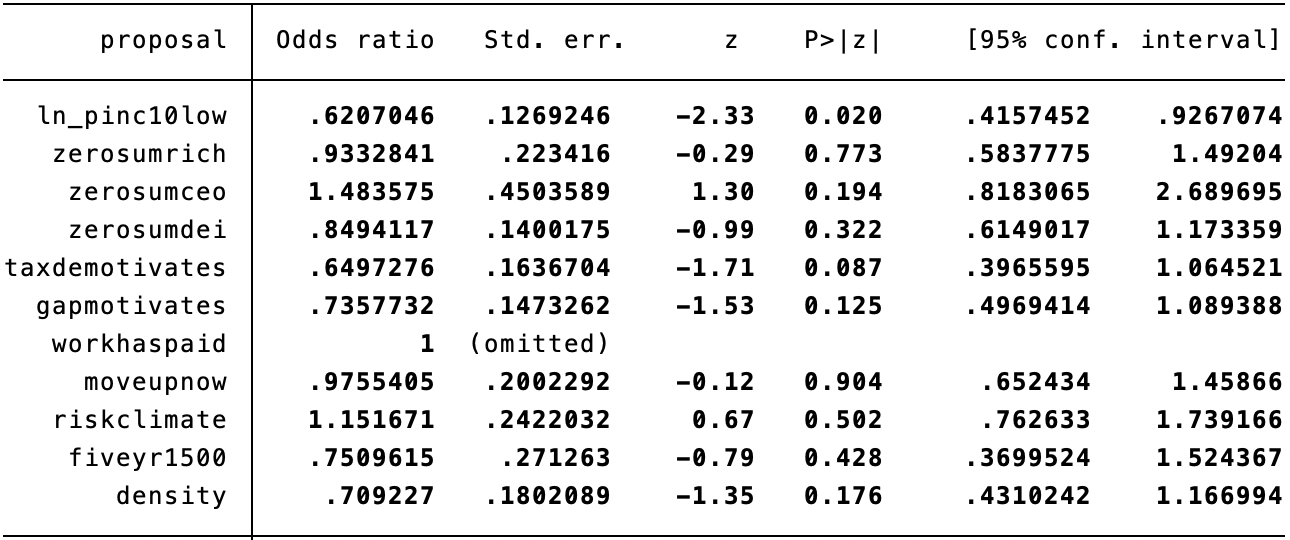
\includegraphics[width=\linewidth]{images/poor notpaid .png}
    \end{subfigure}
    \label{fig:poor-notpaid}
\end{figure}

\begin{figure}[H]
    \centering
    \caption{Wealth tax and downside risk for young (LHS) vs. old (RHS), conditional on belief that hard work has not paid off}
    \begin{subfigure}{.45\textwidth}
        \centering
        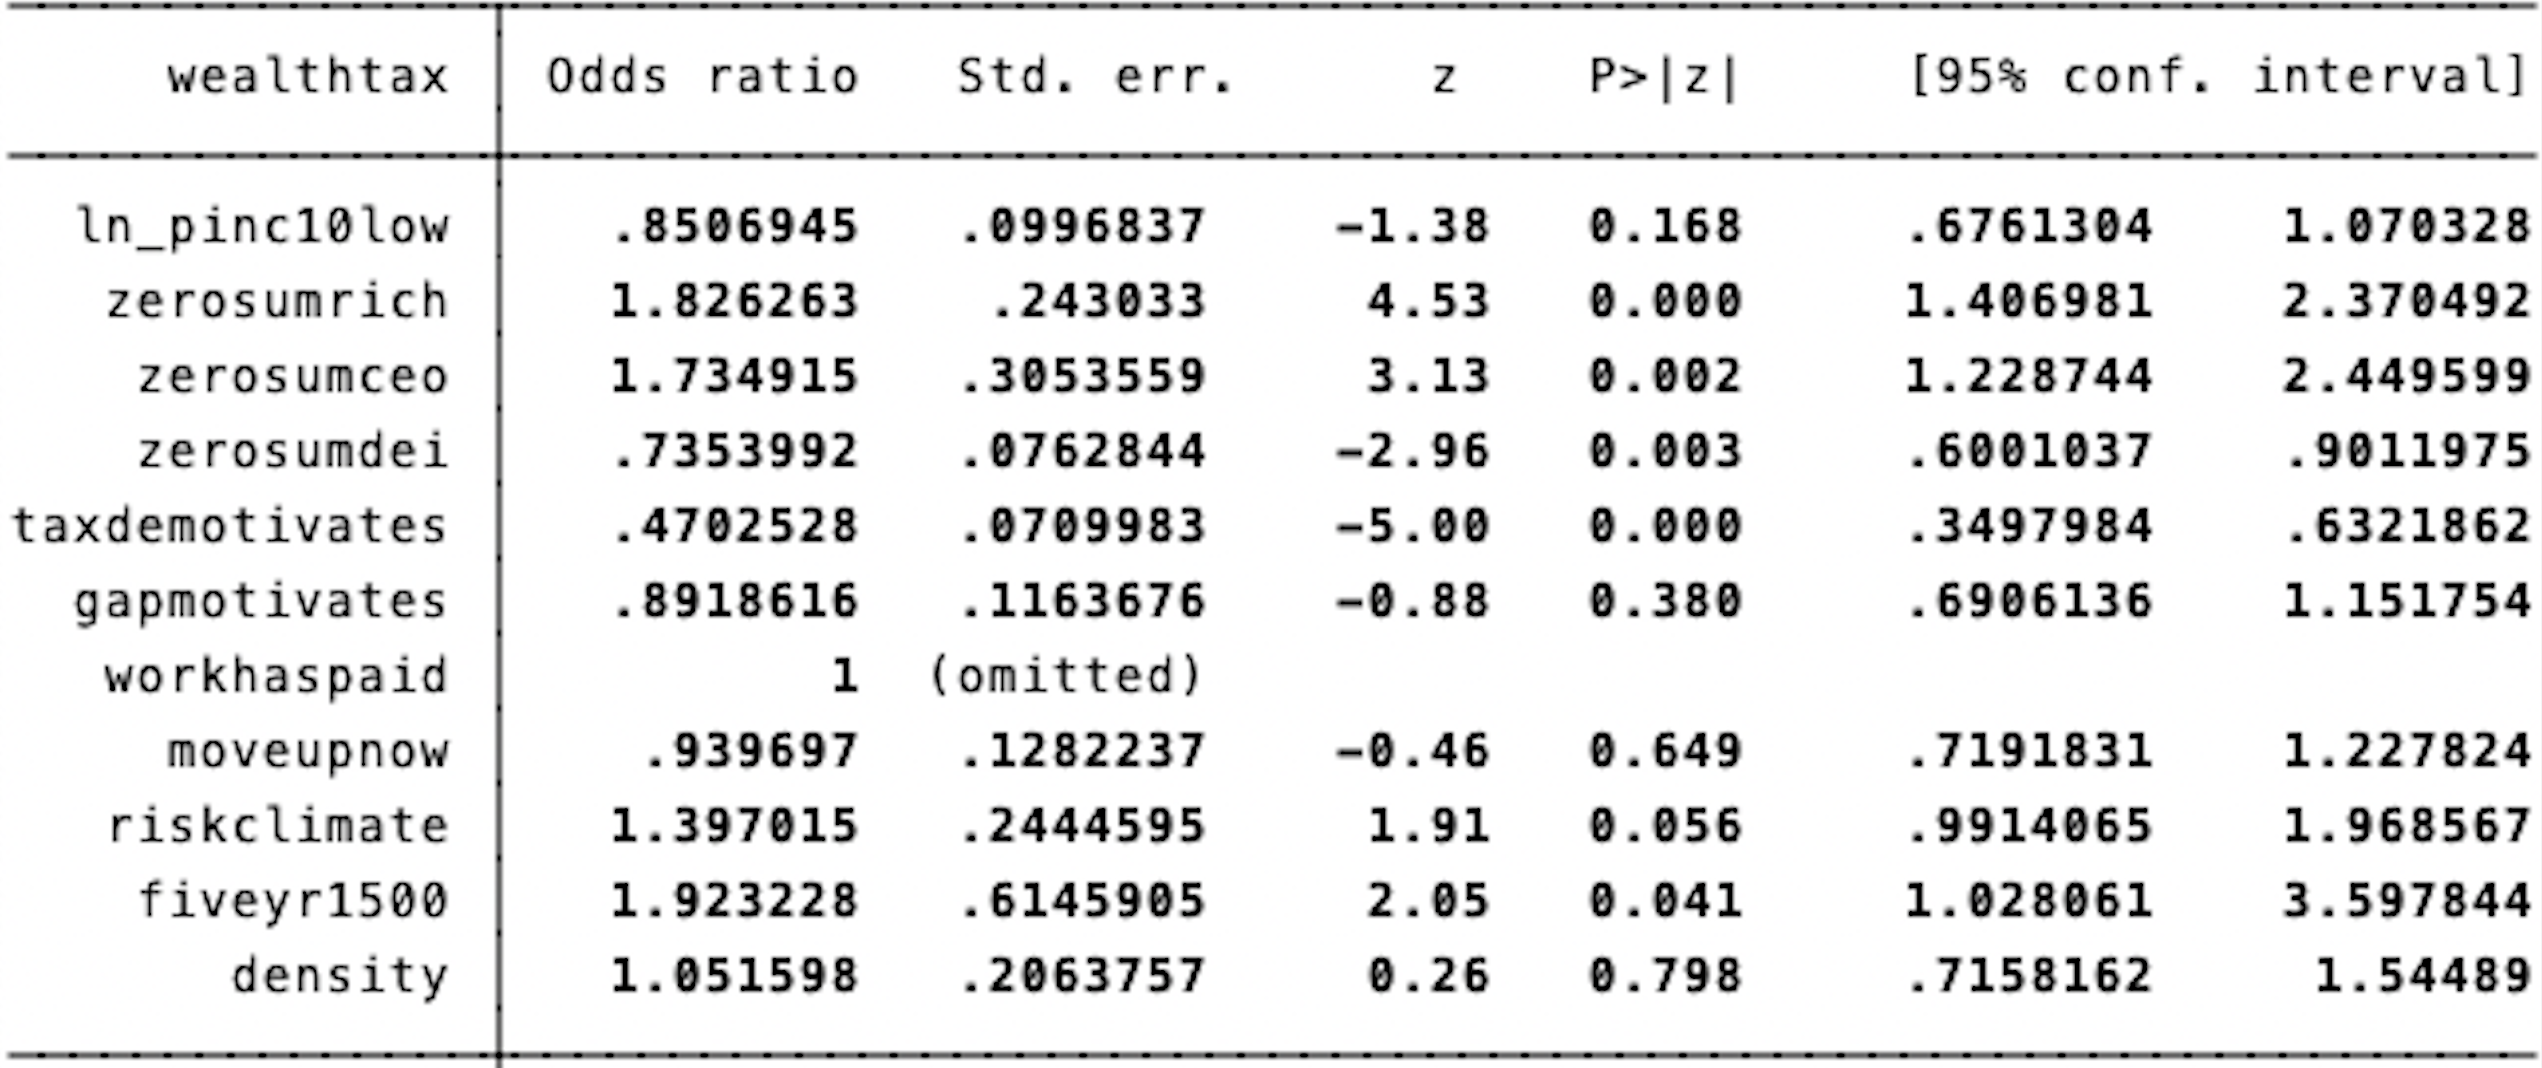
\includegraphics[width=\linewidth]{images/wealthtax notpaid young.png}
    \end{subfigure}
    \begin{subfigure}{.45\textwidth}
        \centering
        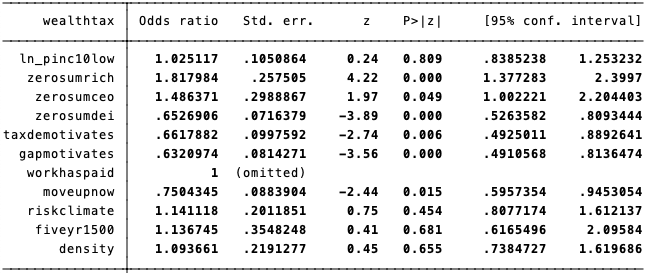
\includegraphics[width=\linewidth]{images/wealthtax notpaid old.png}
    \end{subfigure}
    \label{fig:young-old-wealthtax-notpaid}
\end{figure}

\begin{figure}[H]
    \centering
    \caption{Universal healthcare and downside risk for young (LHS) vs. old (RHS), conditional on belief that hard work has not paid off}
    \begin{subfigure}{.45\textwidth}
        \centering
        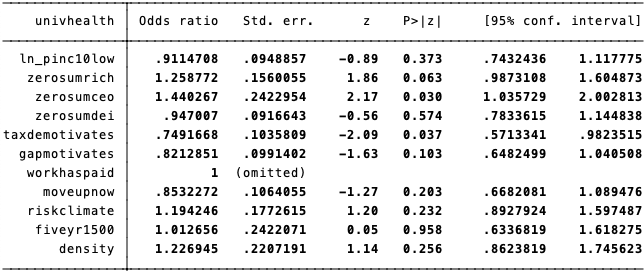
\includegraphics[width=\linewidth]{images/univhealth notpaid young.png}
    \end{subfigure}
    \begin{subfigure}{.45\textwidth}
        \centering
        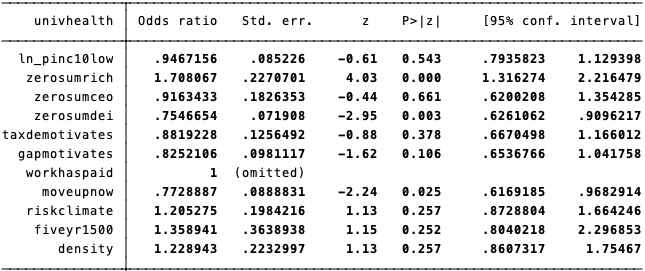
\includegraphics[width=\linewidth]{images/univhealth notpaid old.png}
    \end{subfigure}
    \label{fig:young-old-univhealth-notpaid}
\end{figure}

\begin{figure}[H]
    \centering
    \caption{Funding education and downside risk for young (LHS) vs. old (RHS)}
    \begin{subfigure}{.45\textwidth}
        \centering
        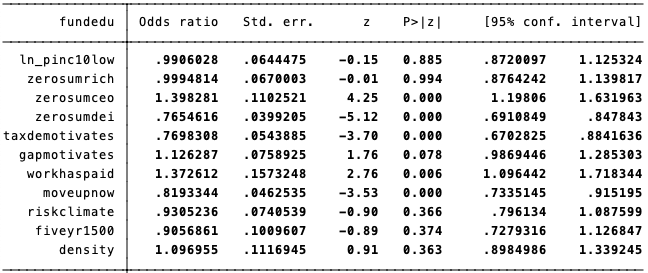
\includegraphics[width=\linewidth]{images/fundedu young.png}
    \end{subfigure}
    \begin{subfigure}{.45\textwidth}
        \centering
        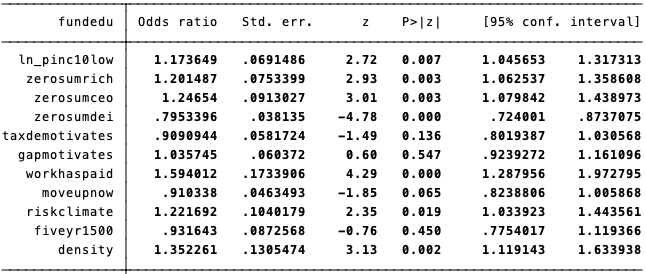
\includegraphics[width=\linewidth]{images/fundedu old.png}
    \end{subfigure}
    \label{fig:young-old-fundedu-notpaid}
\end{figure}

\begin{figure}[H]
    \centering
    \caption{Trade protections and downside risk for young (LHS) vs. old (RHS), conditional on belief that hard work has not paid off}
    \begin{subfigure}{.45\textwidth}
        \centering
        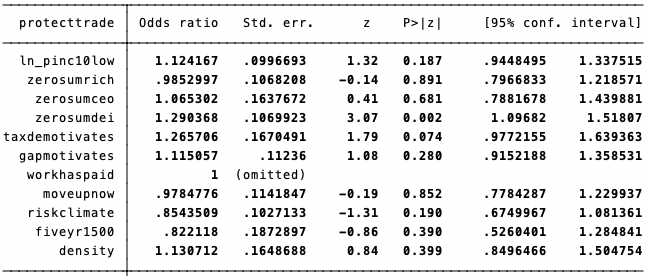
\includegraphics[width=\linewidth]{images/protecttrade notpaid young.png}
    \end{subfigure}
    \begin{subfigure}{.45\textwidth}
        \centering
        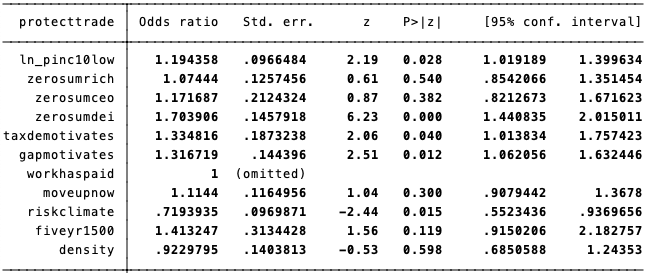
\includegraphics[width=\linewidth]{images/protecttrade notpaid old.png}
    \end{subfigure}
    \label{fig:young-old-protecttrade-notpaid}
\end{figure}


\end{document}
